% Asset ID: A21FunctionsAndGraphsTIKZ-004
% Unit: A21: A2 1 Pure Mathematics
% Topic code: A21-AF
% Related LO IDs: A21-AF-LO006
% Related lesson section: Tricky Modulus Parameter Question
% Source: Chapter 2 Functions and Graphs transcript section on |6 - x| = 1/2 x + k
% Purpose: Show exactly one solution when the line passes through the vertex of y = |6 - x|.

\documentclass[tikz,border=8pt]{standalone}
\usepackage{amsmath}
\usetikzlibrary{arrows.meta}
\begin{document}
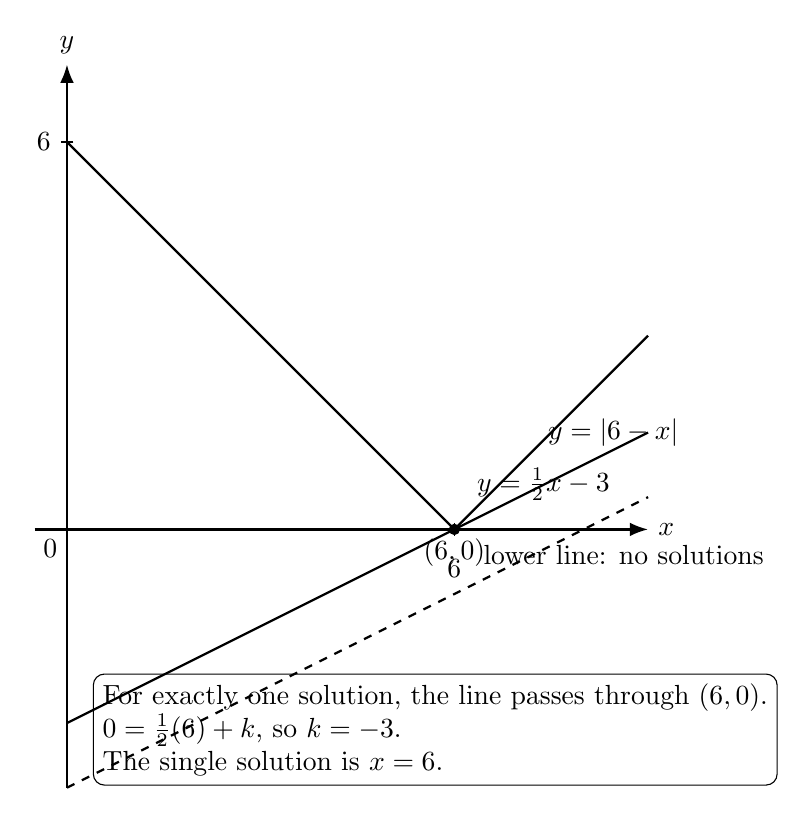
\begin{tikzpicture}[scale=0.82, >=Latex]
\draw[->, thick] (-0.5,0) -- (9,0) node[right] {$x$};
\draw[->, thick] (0,-4) -- (0,7.2) node[above] {$y$};
\draw[thick] (0,6) -- (6,0) -- (9,3);\node[right] at (7.3,1.5) {$y=|6-x|$};
\draw[thick] (0,-3) -- (9,1.5);\node[right] at (6.2,0.7) {$y=\frac12x-3$};
\draw[dashed, thick] (0,-4) -- (9,0.5);\node[right] at (6.3,-0.4) {lower line: no solutions};
\fill (6,0) circle (2.5pt);\node[below] at (6,0) {$(6,0)$};
\draw (6,0.1) -- (6,-0.1) node[below=5pt] {$6$};
\draw (0.1,6) -- (-0.1,6) node[left] {$6$};
\node[below left] at (0,0) {$0$};
\node[draw, rounded corners, align=left, anchor=west] at (0.4,-3.1) {For exactly one solution, the line passes through $(6,0)$.\\$0=\frac12(6)+k$, so $k=-3$.\\The single solution is $x=6$.};
\end{tikzpicture}
\end{document}
